\chapter{Fundamentação Teórica e Trabalhos Relacionados}

Neste capítulo são discutidos os conceitos básicos ao entendimento deste trabalho, abrangendo aprendizagem de máquina, processamento digital de imagens, segmentação de imagens e extração de características.

\section{Aprendizagem de Máquina}

Conforme \cite{alpaydin:2010}, aprendizagem de máquina é uma área da inteligência artificial que estuda métodos computacionais, a fim de obter um determinado conhecimento específico através de experiências. A aplicação prática de aprendizado de máquina inclui o processamento de linguagem natural, diagnósticos médicos, detecção de intrusos, entre outros. Um sistema de aprendizado tem a função de analisar informações e generalizá-las, para a extração de novos conhecimentos.

Segundo \cite{russell:2010}, os tipos de aprendizagem podem ser classificados de acordo com o tipo de \textit{feedback} que recebem do ambiente:

\begin{itemize}
    \item \textbf{Aprendizagem não-supervisionada}: o agente aprende padrões na entrada, embora não seja fornecido nenhum \textit{feedback} explícito. A tarefa mais comum de aprendizagem não-supervisionada é o agrupamento, ou seja, a detecção de grupos de exemplos de entrada potencialmente úteis.
    \item \textbf{Aprendizagem por reforço}: também conhecida como aprendizagem semi-supervisionada. O agente aprende a partir de uma série de reforços - recompensas ou punições.
    \item \textbf{Aprendizagem supervisionada}: o agente observa alguns exemplos de pares de entrada e saída, e aprende uma função que faz o mapeamento da entrada para a saída. 
\end{itemize}

Os problemas de aprendizagem podem ainda ser divididos de acordo com o tipo de saída que demandam:

\begin{itemize}
	\item \textbf{Problemas de classificação}: quando a saída esperada para o problema é uma classe ou categoria, ou seja, um valor discreto;
	\item \textbf{Problemas de regressão}: quando a saída esperada para o é um valor numérico, normalmente contínuo.
\end{itemize}

Um problema de classificação, ou seja, um problema em que o objetivo é atribuir corretamente classes discretas (rótulos) aos exemplos de dados, consiste na determinação de regras e posterior classificação desses exemplos. Este conjunto de regras (classificador) recebe como entrada um vetor de características e oferece como saída uma classe resultante para a instância que as características descrevem, conforme pode ser visto na figura \ref{fig:classificador}.

\begin{figure}[h!]
  \centering
  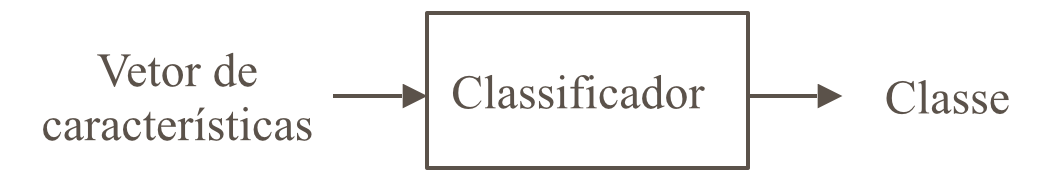
\includegraphics[width=0.7\textwidth]{imgs/classificador}
  \caption{Representação de classificador como uma função de bloco}
  \label{fig:classificador}
\end{figure}

Os tipos de classificadores utilizados neste trabalho serão discutidos com mais detalhes na seção \ref{sec:classificacao}.

O fluxo de uma solução de classificação passa normalmente por três etapas, detalhadas nas próximas seções:

\begin{enumerate}
    \item Filtragem e pré-processamento da entrada;
    \item Extração e seleção de características;
    \item Classificação.
\end{enumerate}


%Os algoritmos utilizados em problemas de classificação podem ser categorizados em:

%\begin{itemize}
%	\item \textbf{Probabilísticos}:
%	\item \textbf{Geométicos}:
%	\item \textbf{Simbólicos}:
%\end{itemize}

% TODO O que são conjuntos de classificadores?
% TODO falar dos essembles e etc.

% TODO O que é reconhecimento de padrões?
% TODO Como reconhecimento de padrões e aprendizagem de máquina se integram?

%Existe uma grande variedade de algoritmos de aprendizagem de máquina propostos na literatura tais como Árvores de Decisão, k Vizinhos mais Próximos (kNN), Redes Neurais Artificiais, Support Vector Machines (SVM), etc. [Santos, 2008]. Além desses métodos individuais, os algoritmos de aprendizagem de máquina podem também ser combinados em conjuntos de classificadores [Dietterich, 2000].

%anto classificadores individuais quanto conjuntos de classificadores são treinados usando vetores de características. Segundo \cite{jain:1989}, o processo de reconhecimento de padrões em imagens normalmente passa por três etapas:
%\begin{itemize}
%    \item Filtragem e pré-processamento da entrada;
%    \item Extração e seleção de características;
%    \item Classificação
%\end{itemize}

\subsection{Filtragem e Pré-processamento}

A etapa de filtragem e pré-processamento é responsável pela escolha e montagem da base de treinamento que será usada no processo de aprendizagem.

%TODO Reaproveitar: Em aprendizado relacionado a imagens, essa etapa é comumente a responsável por normalizar e salientar as características desejadas nas amostras (realce de imagens, filtragem, etc). Nesta etapa, dados irrelevantes, redundantes ou distorcidos são eliminados.

\subsection{Extração de Características}

A extração de características é feita selecionando os atributos oriundos dos dados (imagens, no trabalho em questão), a fim de encontrar as características úteis para o processo de reconhecimento. Essa etapa é crítica ao sucesso do aprendizado, uma vez que bons algoritmos de aprendizado só obtém êxito com uma bom conjunto de características relevantes ao problema.

\subsection{Classificação}\label{sec:classificacao}

Nesta etapa, todas as amostras de treinamento são classificadas e um modelo de aprendizado é gerado. Posteriormente ao processo de aprendizado, é nesta mesma etapa que as amostras não classificadas (ou rotuladas) receberão uma classe dentre as envolvidas no problema. É neste momento que podemos comparar o desempenho de diferentes algoritmos de aprendizado para o conjunto de características escolhidos para representar o problema. Comumente, o percentual de acerto obtido na classificação das amostras não rotuladas é um importante parâmetro para medir a acurácia do método.

São muitos os exemplos de classificadores que existem na literatura. Alguns dos mais utilizados são: classificadores estatísticos, redes neurais artificiais, árvores de decisão, máquinas de vetores de suporte, KNN, etc \cite{jain:1989}.

Os algoritmos utilizados neste trabalho serão discutidos no capítulo \ref{cap:metodologia}

\section{Trabalhos Relacionados}

O trabalho de \cite{dubuisson:2000} apresenta uma técnica de segmentação focada em imagens aéreas coloridas que realiza a segmentações separadamente por cor e textura, para no final unir as duas e chegar a uma segmentação final utilizando um algoritmo de classificação por máxima verosimilhança (\textit{Maximum Likelihood}). O objetivo do trabalho de \cite{dubuisson:2000} é atualização de mapas antigos a partir de imagens recentes, mas as técnicas, se comprovadamente úteis ao problema deste trabalho, podem ser aplicadas em uma pré-classificação de tipos de terreno.

De acordo com \cite{sadgal:2005}, o processamento de imagens digitais que representam cenas naturais requer elaboração substancial em todos os níveis: pré-processamento, segmentação, reconhecimento e interpretação. O trabalho apresentado sugere uma abordagem onde todas essas etapas acontecem em um único nível, e propõe um modelo de visão que tenta generalizar o reconhecimento de objetos utilizando categorização e cooperação.  A solução proposta combina processos estocásticos, dentre os quais Inferência Bayesiana, Campos Aleatórios de Markov, com métodos não estocásticos como Redes Neurais Artificiais. Esta diversidade de métodos é utilizada na segmentação e na extração de características de cores, texturas e formas, que depois são usadas na classificação dos objetos.

A pesquisa realizada por \cite{ahmadi:2013} tem como objetivo fazer segmentação semântica e classificação de imagens aéreas, pixel a pixel. Para tal, diversos classificadores e atributos das imagens são testados, chegando-se a conclusão de que o uso do algoritmo de KNN em características de cor e textura, mais precisamente o filtro de Gabor \cite{fogel:1989} dos canais de matiz, saturação e intensidade (HSV) de cada pixel, obtiveram os melhores resultados, com um desempenho computacional superior aos métodos de baseline.

O trabalho de \cite{ghiasi:2013} realiza segmentação e classificação de tipos de terreno em imagens aéreas através de dois passos: primeiramente a imagem é dividida em superpixels, utilizando a técnica de fluxos geométricos de \cite{levinshtein:2009}; posteriormente, cada superpixel tem suas características de textura e cor extraídas e é classificado através do algoritmo KNN. As características apontadas como mais úteis pelos autores são o Local Binary Pattern Histogram Fourier (LBP-HF) \cite{ahonen:2009} para informações de textura e histograma dos canais RGB para informações sobre cores. O artigo alega conseguir realizar o processo em tempo real, com precisão superior a 95\% em todas as classes utilizadas.

Este trabalho pretende adaptar ou enriquecer os métodos utilizados na literatura, aplicando-os especificamente à segmentação e classificação de imagens aéreas de floresta amazônica, que possui seus desafios característicos, visto que o tipo de terreno e vegetação apresentam padrões diferentes dos vários trabalhos realizados em áreas urbanas ou florestas temperadas.